\documentclass[letterpaper,12pt,fleqn]{article}
\usepackage{matharticle}
\usepackage{siunitx}
\usepackage{pgfplots}
\pgfplotsset{compat=1.14}
\pagestyle{plain}
\begin{document}

\begin{center}
\Large Math-1003b Final Exam
\end{center}

\vspace{0.5in}

Name: \rule{4in}{1pt}

\vspace{0.5in}

This exam is closed book and notes. You may use a scientific calculator;
however, no other electronics are allowed. Calculators may not be shared.
Show all work; there is no credit for guessed answers. All answers must be in
simplified form with no negative exponents. Decimal answers are only acceptable
where requested; otherwise, presence of a decimal value will result in no
credit for the entire problem.

\vspace{1in}

\begin{enumerate}
\item Simplify the following expression:
  \[\left(\frac{x-2}{x^2-3x-18}\right)\left(\frac{3x-18}{x^2-4}\right)\]

  \newpage

\item Simplify the following expression:
  \[\frac{4}{3m}-\frac{1}{m+2}\]

  \vspace{3in}

\item A runner competes in a \SI{2}{mile} race. He runs the first mile
  \SI{1}{mph} faster than the second mile and finishes the first mile
  \SI{3}{minutes} ($\frac{1}{20}$ of an hour) faster than the second mile.
  How fast (in mph) did he run the first mile? For full credit you must show
  the original equation in one variable ($t$) as a difference of rational
  functions ($t_2-t_1=\Delta{t}$) and then solve the equation.

  \newpage

\item Let $f(x)=x^{-\frac{2}{3}}+\abs{x}-3$. Evaluate the function at
  $x=-8$.

  \vspace{1.5in}

\item Sketch (do not plot points) for the following functions:

  \vspace{0.5in}
  
  \begin{enumerate}
  \item $f(x)=\abs{x}$.

    \begin{tikzpicture}
      \draw (-3,0) -- (3,0);
      \draw (0,-3) -- (0,3);
    \end{tikzpicture}

    \vspace{0.5in}

  \item $f(x)=x^3$.

    \begin{tikzpicture}
      \draw (-3,0) -- (3,0);
      \draw (0,-3) -- (0,3);
    \end{tikzpicture}
  \end{enumerate}

  \newpage

\item Use the graph of $K(x)$ to answer the following questions:

  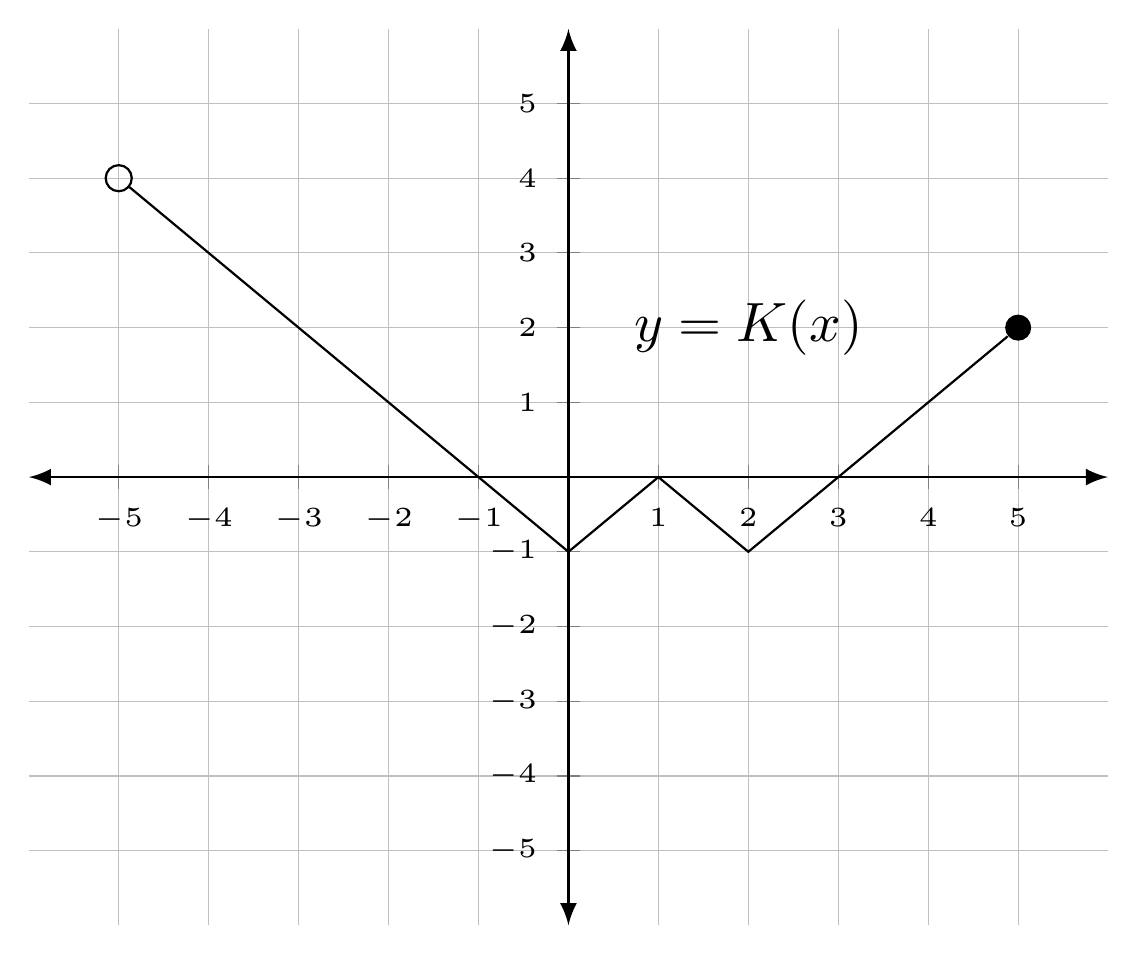
\begin{tikzpicture}[scale=2]
    \begin{axis}[
        xmin=-6,xmax=6,
        ymin=-6,ymax=6,
        grid=both,
        grid style={line width=.1pt, draw=gray!10},
        major grid style={line width=.2pt,draw=gray!50},
        axis lines=middle,
        axis line style={latex-latex},
        xtick={-5,-4,-3,-2,-1,0,1,2,3,4,5},
        ytick={-5,-4,-3,-2,-1,0,1,2,3,4,5},
        ticklabel style={font=\tiny},
      ]
      \node (a) [circle,draw,scale=0.5] at (-5,4) {};
      \node (b) [circle,fill,scale=0.5] at (5,2) {};
      \draw (a) to (0,-1) to (1,0) to (2,-1) to (b);
      \node at (2,2) {$y=K(x)$};
    \end{axis}
  \end{tikzpicture}

  \begin{enumerate}
  \item What is $K(2)$?

    \vspace{0.5in}

  \item What is the y-intercept?

    \vspace{0.5in}

  \item For what values of $x$ is $K(x)=0$?

    \vspace{0.5in}

  \item What is the domain of $K$, in interval notation?

    \vspace{0.5in}

  \item What is the range of $K$, in interval notation?
  \end{enumerate}

  \newpage

\item Let $f(x)=x-4$ and $g(x)=x^2+2$. Perform the
  following operations:
  \begin{enumerate}
  \item $f+g$

    \vspace{1in}
    
  \item $fg$

    \vspace{1in}
    
  \item $\frac{f}{g}$

    \vspace{1in}
    
  \item $f\circ g$

    \vspace{1.5in}
    
  \item $g\circ f$

    \newpage
  \end{enumerate}

\item The area of a picture projected on a wall varies directly as the
  square of the distance from the projector to the wall. If a $\SI{10}{foot}$
  distance produces a picture with an area of $\SI{16}{square feet}$, then what
  is the area of a picture produced with the projection unit is moved to a
  distance $\SI{20}{feet}$ from the wall?

  \vspace{3in}

\item Solve the following inequalities. Your answers must be in interval
  notation:
  \begin{enumerate}
  \item $-6<5x+1\le6$

    \vspace{2in}
    
  \item $5x+1\le-6\ \mbox{or}\ 5x+1>6$

  \end{enumerate}

  \newpage
  
\item Solve the following inequalities. Your answers must be in interval
  notation:
  \begin{enumerate}
  \item $x^2-3x-10>0$

    \vspace{4in}
    
  \item $\frac{x-5}{x+2}\le0$

  \end{enumerate}

  \newpage

\item Solve for $x$:
  \begin{enumerate}
  \item $\abs{\frac{1}{2}x+3}-4=4$

    \vspace{2.5in}
    
  \item $\abs{\frac{1}{2}x+3}-4<4$

    \vspace{2.5in}
    
  \item $\abs{\frac{1}{2}x+3}-4\ge4$

  \end{enumerate}

  \newpage

\item Solve the following system of inequalities graphically. For full credit,
  determine and label the $x$ and $y$ intercepts for each line, sketch the
  two lines using the intercepts, and then select the correct region.
  \[\left\{\begin{array}{l} x-y<2 \\ 3x-2y\ge6 \end{array}\right.\]

  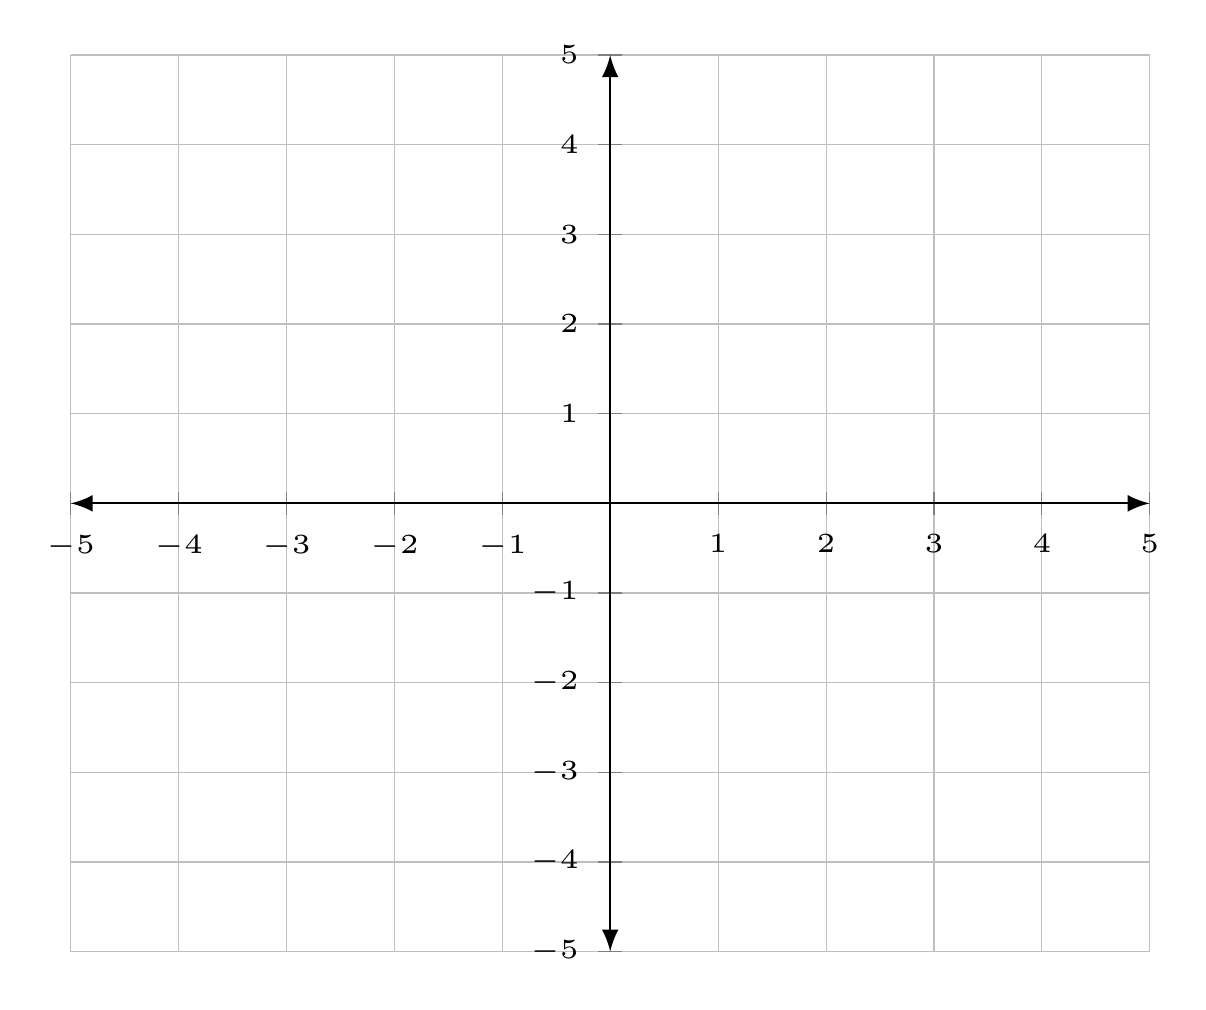
\begin{tikzpicture}[scale=2]
    \begin{axis}[
        xmin=-5,xmax=5,
        ymin=-5,ymax=5,
        grid=both,
        grid style={line width=.1pt, draw=gray!10},
        major grid style={line width=.2pt,draw=gray!50},
        axis lines=middle,
        axis line style={latex-latex},
        xtick={-5,-4,-3,-2,-1,0,1,2,3,4,5},
        ytick={-5,-4,-3,-2,-1,0,1,2,3,4,5},
        ticklabel style={font=\tiny},
      ]
    \end{axis}
  \end{tikzpicture}

  \newpage

\item Simplify (assume all variables are nonnegative):
  \[\left(\frac{16x^{-2}y}{2xy^{-8}}\right)^{\frac{1}{3}}\]

  \vspace{2.5in}

\item Evaluate each of the following. If not possible, say ``not a real
  number'':
  \begin{enumerate}
  \item $16^{\frac{5}{4}}$

    \vspace{0.5in}
    
  \item $-16^{\frac{5}{4}}$

    \vspace{0.5in}
    
  \item $(-16)^{\frac{5}{4}}$

    \vspace{0.5in}
    
  \item $-16^{-\frac{5}{4}}$

    \vspace{0.5in}
    
  \item $\sqrt[4]{16^5}$

  \end{enumerate}

  \newpage

\item Simplify:
  \[5a\sqrt{48a^3}-\sqrt{27a^5}\]

  \vspace{2.5in}

\item Rationalize the denominators of the following:
  \begin{enumerate}
  \item \[\frac{xy}{\sqrt[3]{x^2y^4}}\]

    \vspace{2.6in}

  \item \[\frac{2}{\sqrt{x}-2}\]
    
  \end{enumerate}

  \newpage

\item Solve the following for $x$:
  \[\sqrt{2x+7}-2=x\]

  \vspace{3in}
  
  For problems $18-20$, consider the following general form of a parabola:
  \[y=2x^2+5x-7\]

\item Find the $x$ intercepts by completing the square.

  \newpage

\item Find the $x$ intercepts by using the quadratic formula.

  \vspace{3in}

\item Convert to standard form by completing the square, note the
  $x$-intercepts found above, determine the $y$-intercept, and then sketch the
  graph. The intercepts and vertex MUST be labeled on your sketch for full
  credit!
\end{enumerate}

\end{document}
